%----------------------------------------------------------------------------
\section{Javaslat a kockázatok kiszűrésére}
\label{sec:6}
%----------------------------------------------------------------------------

\subsection{Adversarial módszerek}

A korábban vizsgált megközelítéssel sajnos nem sikerült jó eredményeket elérni. A modell robusztusságából adódóan néhány jellemző kivételével nem romlik a modell pontossága, és a hálózat effektus feltételezés sem bizonyult helyesnek. Következő próbálkozás az adversarial attack módszerek irányába indult. Adversarial examplenek nevezzük azt a mintát, amelyet, ha kis mértékben módosítunk képes becsapni egy adott machine learning modellt. Ezt a gyakorlatban egy kis mértékű pontosan kiszámított zaj hozzáadását jelenti, miközben a modell hibáját maximalizálja. 

Annak érdekében, hogy belássuk, működhetnek az ilyen módszerek azt tűztem ki célul, hogy mutassam be néhány félig manuálisan készített példán keresztül, hogy az arclenyomatok kis mértékű módosításával be lehet csapni a random forest classifier modellünket. Ehhez készítettem egy újabb algoritmust, amelyet előbb Iris dataseten teszteltem a könnyebb értelmezhetőség érdekében, majd miután működött áttértem az arclenyomat vektorok használatára.

Az algoritmus mögöttes ötlete abból ered, hogy ha megvizsgáljuk az egyes döntési fákat, találhatunk olyan elágazásokat (feltételeket) ahol egy adott arclenyomat vektor jellemzőinek értéke a döntési küszöbértékhez meglehetősen közeli értéket vesz fel. Az ilyen esetekben ezeknek a jellemzőknek kis módosításával el lehet érni azt, hogy a döntési fa feltétele átbillenjen, és másik útvonalon halad a következő elágazásig. Ez a módosítás önmagában még nem garantálja azt, hogy a döntési fa kimenete megváltozik, mivel előfordulhat, hogy a kitérítés után egy másik levélre jut, ami ugyanazt az eredményt adja, mint az eredeti kimenet. Ezt szemlélteti a következő példa.

\begin{figure}[ht]
	\centering
	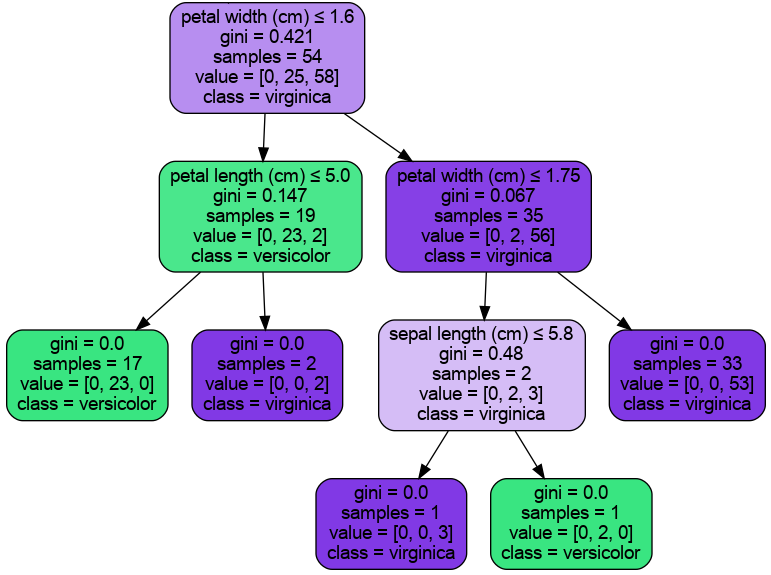
\includegraphics[width=0.9\columnwidth]{figures/adverse_tree_graph.png}
	\caption{Döntési fa részlete, ami az Iris datasetre lett betanítva.}
	\label{fig:iris_tree}
\end{figure}

Tegyük fel, hogy az általunk vizsgált mintában a petal width jellemző értéke 1,55 cm, petal length értéke 4,5 cm. Ezt a mintát a \ref{fig:iris_tree}. ábrán látható döntési fa alap esetben ``versicolor'' kategóriába sorolná. A döntési fa a legfelső elágazásnál petal width $\le$ 1.6 cm feltétel szerepel. Belátható, hogy a bemeneti érték kis módosításával (1.55 + 0.05) átbillenthető a feltétel teljesülése, és az eredeti bal ág helyett jobb ág irányába halad tovább a döntéshozatal, ezzel potenciálisan téves predikcióra vezethető a fa. Azt is láthatjuk ebben a példában, hogy ha a mintánkban a sepal length jellemző értéke nagyobb mint 5,8 cm, akkor újból ``versicolor'' levélre jutunk, tehát előfordulhat, hogy hiába tévesztettük meg a döntési fát egy ponton, a fa predikciója továbbra is változatlan marad.

A véletlen erdő sok döntési fát tartalmaz, amelyek mind képeznek egy-egy szavazatot az egyik kimenetre, ezért egyetlen fa becsapása legtöbb esetben nem elegendő a teljes véletlen erdő kimenetének módosítására, így a bemeneti arclenyomat vektor olyan módosítása szükséges, ami egyidejűleg több döntési fa predikcióját is képes eltéríteni.

\subsubsection*{Adversarial módszer fejlesztése Iris adathalmazon}

Az Iris dataseten betanított random forest classifieren a korábbihoz hasonlóan egy rekurzív függvényt használtam, ami végighalad az erdőben található egyes döntési fákon, és az elágazásoknál vizsgálja az adott feltételhez tartozó jellemző bemeneti értékét, és küszöbértékét. Az algoritmus első verziója egy adott bemenetre keresi azokat a küszöbértékeket, amelyek a bemenettől maximum 10\%-kal térnek el. Ezeknél a feltételeknél van lehetőségünk kis módosítással megtéveszteni a fát. Az ilyen eseteknél a program kiírja melyik fáknál, és melyik jellemző értéknél van megfelelően kis eltérés a küszöbértékhez képest.

\begin{lstlisting}[caption={A döntési azon elágazási pontjai, amelyek kis jellezőmódosítással átbillenthetőek.}]
Tree: 0 out: 1  feature: PL  4.9 <= 4.85, diff: -0.05
Tree: 1 out: 1  feature: PL  4.9 <= 4.95, diff: 0.05
Tree: 2 out: 1  feature: PW  1.5 <= 1.55, diff: 0.05
Tree: 2 out: 1  feature: PL  4.9 <=  5.0, diff:  0.1
Tree: 3 out: 1  feature: PL  4.9 <= 4.95, diff: 0.05
Tree: 4 out: 1  feature: PL  4.9 <= 4.95, diff: 0.05
Tree: 5 out: 1  feature: PL  4.9 <= 4.95, diff: 0.05
(*@\raisebox{-1pt}[0pt][0pt]{$\quad\vdots$}@*)
Tree: 99 out: 1  feature: PW  1.5 <= 1.55, diff: 0.05
\end{lstlisting}

Az eredményeket megpróbáltam valamilyen módon összesíteni, de voltak esetek mikor a küszöb érték alatt volt a jellemző értéke kicsivel, volt mikor fölötte. Az könnyen látható volt, hogy a petal length feltétel szerepelt a 100 fából leggyakrabban, így annak a módosításával próbálkoztam.

A módszer szemléltetésére kerestem egy mintát, ahol a véletlen erdő fái egyértelműen döntöttek az egyik osztály mellett, és a bemenet kis módosításával próbáltam elérni, hogy minél több fa téves predikcióra jusson. Az alábbi mintánál eredetileg a 96 szavazott a ``versicolor'' osztályra, majd egyetlen jellemző viszonylag kis módosítással (petal width 4,9-ről 5.05-re lett növelve) sikerült elérni, hogy a fák többsége ``virginica'' osztályra szavazzon.

\begin{lstlisting}[caption={A véletlen erdő kimenetének manipulációja.}]
Eredeti értékek:
[6.9 3.1 4.9 1.5]
Módosított értékek:
[6.9  3.1  5.05 1.5 ]
Módosítás mértéke:
0.88%

Fa szavazatok:
módosítás előtt [ 0. 96.  4.]
módosítás után  [ 0. 40. 60.]
\end{lstlisting}

\subsubsection*{Adversarial módszer arclenyomat vektorokon}

Az Iris datasetes példán elért eredmények után az algoritmus fejlesztését az arclenyomat vektorokról készült adathalmazon folytattam. Az algoritmus működése során továbbra is végighalad a döntési fán és a bemenet értékeitől függően lép egyik elágazásról a következőre. Ennél a verziónál is detektáltam az olyan elágazásokat, ahol a bemeneti érték egy előre definiált tartományon belül tér el a küszöbértéktől. Minden alkalommal, mikor detektál az algoritmus egy ilyen elágazást, az elágazás mindkét ágán folytatja a fa feltérképezését egészen addig, amíg levél csomóponthoz nem jut. A levélhez eljutva megnézi, hogy az adott levélhez tartozó kimeneti osztály megegyezik-e a mintához tartozó címkével, vagy sem.

Itt az az elgondolás, hogy minden esetben mikor könnyen átbillenthető csomóponthoz jutunk, eldönthetjük, hogy melyik úton érdemes tovább haladni. Az egyes lehetséges utakat feltérképezve ki tudjuk választani azt az utat, ami téves predikcióhoz vezet, illetve, ha több ilyen út van akkor ki tudjuk választani azt, amelyikhez a legkisebb beavatkozás szükséges. 

Az algoritmus végigmegy a véletlen erdő összes döntési fáin, kivéve azokat, amelyek alapból is téves predikciót adnak, mivel ezeken nem kell módosítanunk.

\begin{lstlisting}[caption={Algoritmus futtatása egy adott arclenyomat vektorra.}, label=lst:tree_diffs]
Tree: 4, output: 3
		f10  diff: -0.0267
Tree: 4, output: 2
		f88  diff: -0.04035
Tree: 9, output: 3
		f77  diff: -0.02279
Tree: 11, output: 3
		f93  diff: 0.002902
		f57  diff: -0.008323
		f82  diff: -0.007353
Tree: 11, output: 3
		f93  diff: 0.002902
		f57  diff: -0.008323
		f91  diff: 0.02286
(*@\raisebox{-1pt}[0pt][0pt]{$\quad\vdots$}@*)
Tree: 48, output: 1
		f93  diff: 0.002753
\end{lstlisting}

Az algoritmus lefuttatható egy adott arclenyomat vektorra. Lefuttatás során a \ref{lst:tree_diffs}. kódrészlethez hasonló információt kapunk. Eredményül egy listát kapunk, ami felsorolja azokat a fákat a véletlen erdőn belül, amelyek kis (10\% alatti) input módosítással megtéveszthetőek. Fel van tüntetve a fa sorszáma, illetve a fa megtévesztés utáni predikciója (ennél a példánál helyes predikció 0 lenne.) Egy fához fel vannak sorolva azok a jellemzők amelyeket módosítani kell a fals predikció eléréséhez, ahol a ‘diff’ érték mutatja a szükséges módosítás mértékét. Ha több jellemző van felsorolva, például Tree 11-nél akkor azok a módosítások ÉS kapcsolatban állnak egymással.

Megfigyelhetjük ezen a példán, hogy egy fához több téves predikció is tartozhat, attól függően, hogy melyik jellemzők értékét változtatjuk. Például a Tree 4 esetén elérhetünk 3-mas vagy 2-es predikciót is. Az is előfordulhat, hogy egy döntési fán belül több útvonal vezet egy téves predikcióhoz, például Tree 11 esetén háromféleképpen kaphatunk 3-mas predikciót. Ilyenkor a kisebb módosítást igénylő út a preferált. 

Jelenleg az algoritmus félig automatikus működésű. A lefuttatás során nem fog módosítani az eredeti mintán, azt manuálisan kell elvégezni. Ez az egyik terület, ahol tovább szeretném fejleszteni ezt a megoldást, hogy képes legyen kiszámolni az optimális átalakítást, ahol a legkisebb zaj hozzáadásával megtéveszthető a véletlen erdő becslése. Jelenleg kézzel lehet összeválogatni az egyes jellemzők módosításait, és az alapján összerakni egy zaj vektort. A feladat nehézségét az adja, hogy lehetnek ellentmondásos feltételek (egyik fa növelni szeretné a jellemző értékét, másik pedig csökkenteni), illetve az is előfordulhat, hogy egy jellemző módosítás hatására az egyik fánál korábbi rossz predikció átvált helyesre. Az jellemző módosítások optimális kombinációjának megtalálása nem egyszerű feladat.

\begin{lstlisting}[language=python, caption={Korábbi elemzés alapján manuálisan elvégzett jellemző módosítások.}, label=lst:tree]
# feature modositasok
x_ = x.copy()

x_[:,10] += -0.0268  # Tree 4, Tree 17
x_[:,77] += -0.0228  # Tree 9
x_[:,43] += -0.02737  # Tree 13, 29, 31
x_[:,8] += 0.02539  # Tree 24
x_[:,88] += -0.0314  # Tree 35
x_[:,105] += -0.02175  # Tree 37
x_[:,44] += 0.02302  # Tree 41

print('tree votes:')
print(count_votes(x))
print(count_votes(x_))

# kimenet:
'''
tree votes:
[30. 4. 3. 13.]
[20. 4. 4. 22.]
'''
\end{lstlisting}

A \ref{lst:tree}. kódrészleten láthatjuk, hogyan végezhető el a korábban megállapított jellemzők módosítása. Az eredeti arclenyomat vektor értékeit az ``x'' változó tárolja. A random forest classifier 50 fából áll, melyek közül 30 fa eredetileg 0 predikciót képez. Egy-egy jellemző módosításnál kommentben megneveztem azokat a fákat, amelyeknek a módosítás hatására átváltanak a helyes (0) predikcióról egy másik értékre. Összesen 10 fa megtévesztésével elérhettük azt, hogy a teljes erdő téves predikciót produkál a módosított mintára. 

Fontos még megjegyezni, hogy összességében elég kis módosítással sikerült elérni ezt az eredményt. Az arclenyomat vektor 128 jellemző közül elegendő volt 7-et kiválasztani, és azokat is maximum 10\%-ban módosítani. A feltételezésem az, hogy ez a módosítás elegendően specifikus és kis méretű, hogy ezzel még megőrizhető egy arclenyomat vektorok alapján betanított identifikációs modell pontossága, de ezt még nem teszteltem le.

Összefoglalva, eleinte a hálózat effektus feltételezést vizsgáltam, ami végül nem vezetett eredményre. Bemutattam a hipotézis mögött rejtő gondolatmenetet és a kísérleteket. Később az adversarial attack jellegű algoritmus fejlesztésével foglalkoztam. Bemutattam a döntési fák vizsgálatának módszerét és implementálását. Részleteztem az algoritmus fejlesztésének menetét, az egyszerűbb feladatok megoldását, majd az arclenyomat vektorokon elért eredményeket. Jelenleg az algoritmus félig automatikus működésű, azaz a döntési fák elemzése után kézzel kell összeállítani az arclenyomat vektorok módosítását. Az egyik főbb továbbfejlesztési irány az lenne, hogy az algoritmus képes legyen közel optimális zaj generálására, amellyel a véletlen erdő predikciója becsapható.

Ezt az eredményt a munkával töltött első félév végére értem el, 2021 tavaszán. 2021 júniusban megjelent egy új preprint a Stanford Egyetemről, amiben a szerzők az általam bemutatott adversarial módszerhez hasonló adatvédelmi eszközöket véleményezik \cite{radiya2021data}. A szerzők szerint az ilyen módszerek hatása limitált. Az egyik érvük az, hogy ha az adatot  adversarial módszerekkel védjük, és azokat a támadó megszerzi, akkor a támadónak lehetősége van adaptálnia a modelljét, azaz a védett arclenyomatokat felhasználva képes újratanítania a modelljét, ami ellenálló lesz a védekezési mechanizmussal szemben. 

Erre hoznak egy példát: a Fawkes rendszert \cite{shan2020fawkes}, ami a felhasználói számára erős védelmet ígér az arcfelismerő rendszerekkel szemben. A Fawkes a felhasználók által feltöltött képek kisebb perturbálásával érik el azt, hogy az arcfelismerő rendszerek tévesen azonosítsák a képen látható személyeket. A Fawkes rendszer hatékonyan működött és elhíresült, több mint 500 000 felhasználó letöltötte. Ennek ellenére később a Microsoft arcfelismerő rendszerét úgy módosították, hogy a Fawkes védelmével szemben ellenálljon. A Fawkes fejlesztői erre kiadtak egy új frissítést, ami újból védelmet tud nyújtani a Micosofttal szemben, amiről a Fawkes weboldalán olvashatunk \cite{fawkes_update}.

Mivel mindkét fél képes adaptálni a támadó / védekező módszereit, így ez egy ``fegyverkezési versenyre'' vezethet. Viszont ebben a versenyben a támadónak jelentős előnye van. A Fawkes példában hiába fejlesztenek ki egy újabb verziót a védelmi rendszernek, a támadó már sikeresen feltörte a régi verzió által védett képeket, így azok már nincsenek védve.

A \cite{radiya2021data} szerzői szerint ez az adversarial módszerek csak ideiglenes védelmet tudnak nyújtani, de nem adnak hosszútávú megoldást. Szerintük megoldásnak az arcfelismerő rendszerek jogszabályokkal való korlátozása jelenthet. 

\subsection{Kriptográfiai módszerek}

% 4-5 oldal
% \begin{itemize}
% 	\item cancelable biometrics
% 	\item motiváció, titkosítási módszerek előnyei (0.5 - 1 oldal)
% 	\item klasszikus hashelés, LSH, random projekció (1 - 1,5 oldal)
% 	\item klasszikus titkosítási, homomorfikus, hogy képzelhető el arcfelismerésnél  (1-1,5 oldal)
% \end{itemize}

A korábban bemutatott módszerek célja az volt, hogy a \ref{sec:tamado}. fejezetben bemutatott támadót feltételezve, egy arcfelismeréshez használt központi arclenyomat adathalmaz feltörése esetén az arclenyomatokból ne lehessen érzékeny adatokat kinyerni. Ennek érdekében olyan módszereket vizsgáltam, amelyek az arclenyomatok kis módosításával meggátolná a személyes adatok szivárgását. Ebben a fejezetben egy másik megközelítést, olyan titkosítási módszereket mutatok be, amelyek alkalmazhatóak az arcfelismerés területén.

Egy arclenyomat adathalmaz feltörése azért kritikus biztonsági szempontból, mert az ember arcáról készült arclenyomatok nem változnak idővel. Míg felhasználói jelszavak kiszivárgása esetén van lehetőség a jelszó módosítására, arcfelismerő rendszerek esetén nincs lehetőség arra, hogy valaki megváltoztassa az arclenyomatát. Emellett kockázatot jelen az is, hogy ugyanaz a biometrikus azonosítót több hitelesítési rendszerben is használhatnak. Ha az egyik alkalmazás kiszivárogtatja a biometrikus azonosítót, az összes többi rendszert veszélyezteti, ami ugyanazt a biometrikus adatot használja.

A titkosítási módszerek lényege az, hogy az arclenyomatokat nem eredeti formájukban tároljuk, hanem titkosított formában. A biometrikus adatokat valamilyen módszerrel áttranszformálják, majd transzformált állapotban tárolják. A transzformáció lehet invertálható, vagy nem invertálható (azaz végleges). A titkosítás módjára léteznek biometrikus sablonvédelmi módszerek \cite{patel2015cancelable}, amelyeket biometrikus adatok (pl. ujjlenyomat, arclenyomat) tárolására fejlesztettek ki. Ezeket mutatom be részletesebben a továbbiakban.

% visszaalakítás összehasonlításhoz

% kiszivárgás nem jelent problémát mert újat lehet generálni

\subsubsection{Hashelési módszerek}

% ezt ki lehet egészíteni azzal, hogy különböző cégek különböző hash fv-t használhatnak
Az arclenyomatok titkosításához egy egyszerű és bevált módszer lenne a szabványos titkosítási technikák, mint például a hash függvények alkalmazása. A hash függvények a biometrikus adatok védelmére lehet használni, mivel hesselés során az adat végleges átalakításon megy keresztül. A hash függvényeket szinte lehetetlen invertálni, így ha a hesselt arclenyomatok kiszivárognak, azokból az eredeti arclenyomatokat nem lehet visszanyerni. Emellet előnye még a módszernek az, hogy különböző applikációk eltérő hash függvényt használnának, így ha az egyik applikáció adatbázisát feltörik, az nem jelent veszélyt a többi applikációra.

Egy probléma van a klasszikus hesselési eljárásokkal, hogy a hash függvény kimenete már kicsiben eltérő bemenetre is teljesen eltérő lesz. Ez azért probléma, mert a legtöbb biometrikus adat esetén, beleértve az arclenyomatokat is, a környezeti hatások befolyásolhatják az arclenyomatok pontos értékeit. Például egy személyről eltérő fényviszonyokban, vagy más szögekből készült arcképekből származtatott arclenyomatok kis mértékben eltérnek egymástól. Az egymáshoz közeli arclenyomatok hesselés során nagyban különböző kimenetet kapnak, és emiatt nem alkalmasak összehasonlításra \cite{patel2015cancelable}. 

Ez a probléma megoldható, ha egy olyan hash függvényt használunk, ami a közeli pontoknak azonos kimenetet képez. Az ilyen módszereket lokalitás érzékeny hash függvényeknek hívjuk (angol szakirodalomban locality sensitive hashing, röviden LSH) amelyeket használnak például képek hasonlóságának mérésére \cite{jing2008visualrank}. A lokalitás érzékeny hash függvények létezését a Johnson-Lindenstrauss lemma mondja ki, miszerint több magas dimenziójú térbeli pont leképezhető alacsonyabb dimenziójú térbe oly módon, hogy bármely két pont közötti távolság közel azonos marad  \cite{johnson1984extensions}. Az LSH függvények segítségével adatpontok csoportosíthatóak, hiszen a hasonló bemeneteket nagy valószínűséggel azonos csoportba sorolja az algoritmus. A \ref{fig:lsh}. ábrán látható a különbség a klasszikus hashelés és az LSH között.

\begin{figure}[ht]
	\centering
	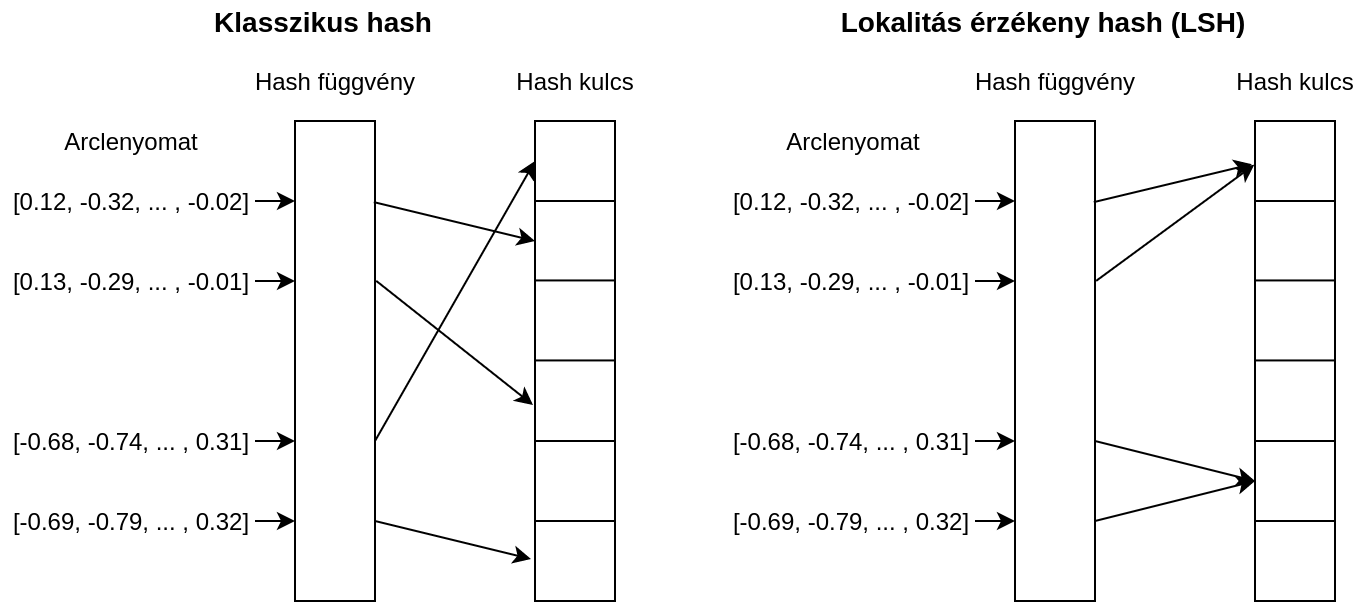
\includegraphics[width=1\columnwidth]{figures/lsh.png}
	\caption{Bal oldalon a klasszikus hesselés látható, jobb oldalon az LSH.}
	\label{fig:lsh}
\end{figure}

Az LSH módszerek már alkalmasak lehetnek arcfelismerő rendszerek esetén az arclenyomatok biztonságos tárolására. Az arcfelismerő rendszer tárolja a hash függvényt, illetve a személyek arclenyomatait hesselt formában. Hitelesítés során az ismeretlen személy arcképéből az arcfelismerő rendszer arclenyomatot képez, amelyet a rendszerben tárolt LSH függvénnyel hesselik, majd összevetik a tárolt hessekkel. Ha a bemeneti képből képzett hash megfelelően közel van az egyik eltárolt sablonhoz, akkor sikeres a hitelesítés.


% A simple approach would be to use standard encryption techniques such as hash func- tions or encryption to enhance the privacy. Hash functions have been used to protect biometric templates in which one-way func- tions are used to compute a digest. Even though these functions are almost impossible to invert, they produce a significantly differ- ent digest even with minor changes in the input. In practice, all biometric templates change with environmental conditions. For instance, face and iris biometrics are significantly affected by illu- mination variations. Therefore, these functions cannot be used directly in practice despite being theoretically very strong as they apply only to exact data.

\subsubsection{Titkosítási módszerek} % kripto kulcs alapú

% klasszikus titkosítási módszer hogy működik
% probléma: összehasonlításhoz vissza kell állítani
% erre megoldás a homomorfikus titkosítás

% titkosító algoritmus és kulcs segítségével titkosított adat -> csak az tudja olvasni aki rendelkezik az olvasáshoz szükséges kulccsal

% when data are encrypted, they need to be decrypted to carry out matching. This creates a possible attack point to get access to the decrypted templates. 

A titkosítás vagy rejtjelezés olyan kriptográfiai eljárás, amellyel valamilyen adatot egy titkosító algoritmus kulcs segítségével átalakítja olyan formára, amely ember számára olvashatatlan. Az adat olvasását csak az teheti meg, aki rendelkezik az olvasáshoz szükséges kulccsal. A titkosított adatok gyakorlatban szinte feltörhetetlenek. Ennek ellenére arclenyomatok védelmére mégsem ideális a klasszikus titkosítási módszerek. 

Ennek oka az, hogy az arcfelismerő rendszer működéséhez szükséges az azonosítandó személy arclenyomatát a rendszerben tárolt arclenyomatokkal összevetni valamilyen módszerrel, például az arclenyomatok közötti euklideszi távolság alapján. Ha az adatbázisban tárolt arclenyomatok titkosítva vannak, akkor azokat először szükséges dekódolni az összehasonlításhoz, mert a titkosított adatokon közvetlenül nem tudjuk elvégezni a szükséges műveleteket. 

A titkosított adatokkal általánosságban az a probléma, hogy ahhoz, hogy műveleteket végezzünk rajtuk dekódolni kell. Dekódolással viszont egy lehetséges támadási pont nyílik meg a rendszerben, ahol lehetséges hozzáférni az eredeti adatokhoz.

Van erre a problémára egy hatékony megoldás amit homomorfikus titkosításnak hívnak. A homomorfikus titkosítás egy publikus kulcsot használ az adat titkosítására. A klasszikus titkosítási módszerektől eltérően a homomorfikus titkosítással lehetséges a titkosított adatokon matematikai műveleteket végezni. A titkosított adatokon végzett műveletek eredménye is titkosított adat lesz, amelyet dekódolva ugyanazt az eredményt kapjuk, amit a titkosítatlan adatokon elvégzett ugyanezen műveletek eredményeztek volna. Így a hitelesítési fázisban nincs szükség a titkosított adatokat dekódolni, azokon közvetlenül el lehet végezni az összehasonlítást. 

A homomorfikus titkosításnak három fő típusa van:

\begin{itemize}
	\item \textbf{Partially homomorphic encryption}: Ebben az esetben csak bizonyos matematikai műveleteket lehet végrehajtani a titkosított adatokon.
	\item \textbf{Somewhat homomorphic encryption}: Korlátozott számú műveletet támogat, amelyek csak meghatározott számú alkalommal hajthatóak végre.
	\item \textbf{Fully homomorphic encryption}: A teljesen homomorfikus titkosítás (FHE) minden műveletet támogat, és a műveletek korlátlan számmal hajthatóak végre. Ez a legerősebb típusa a homomorfikus titkosításnak. 
\end{itemize}

A homomorfikus titkosításnak jelenleg az a legnagyobb hátránya, hogy magas a számításigénye az eljárásnak, ezért elég lassú, és emiatt nem praktikus még az alkalmazása. Az arcfelismerő rendszereknél alkalmazható lehet egy olyan részlegesen homomorfikus titkosítást alkalmazni, ami gyorsabb működésű mint az FHE támogatja az összeadást, így távolságméréshez euklideszi távolság helyett lehet például Manhattam távolságot használni.

% A homomorf titkosítás széles körű elterjedésének legnagyobb akadálya az, hogy még mindig nagyon lassú – olyan lassú, hogy még nem praktikus sok alkalmazáshoz. azonban

% Just like other forms of encryption, homomorphic encryption uses a public key to encrypt the data. Unlike other forms of encryption, it uses an algebraic system to allow functions to be performed on the data while it’s still encrypted. Then, only the individual with the matching private key can access the unencrypted data after the functions and manipulation are complete. This allows the data to be and remain secure and private even when someone is using it. 

% There are three main types of homomorphic encryption: partially homomorphic encryption (keeps sensitive data secure by only allowing select mathematical functions to be performed on encrypted data); somewhat homomorphic encryption (supports limited operations that can be performed only a set number of times); fully homomorphic encryption (this is the gold standard of homomorphic encryption that keeps information secure and accessible).

% The biggest barrier to widescale adoption of homomorphic encryption is that it is still very slow—so slow it’s not yet practical to use for many applications. However

% A homomorf titkosításnak három fő típusa van: részlegesen homomorf titkosítás (biztonságban tartja az érzékeny adatokat azáltal, hogy titkosított adatokon csak bizonyos matematikai függvények végrehajtását engedélyezi); kissé homomorf titkosítás (korlátozott műveleteket támogat, amelyek csak meghatározott számú alkalommal hajthatók végre); teljesen homomorf titkosítás (ez a homomorf titkosítás aranystandardja, amely biztonságosan és hozzáférhetően tartja az információkat). 
% A homomorf titkosítás széles körű elterjedésének legnagyobb akadálya az, hogy még mindig nagyon lassú – olyan lassú, hogy még nem praktikus sok alkalmazáshoz. azonban